\documentclass[12pt,a4paper,oneside]{article}
%\documentclass[12pt,a4paper,oneside,twocolumn]{article}
\usepackage{pagestyle}
\usepackage{codestyle}

% Report hand-in date
\DTMsavedate{date}{2024-03-29}

\title{
    \Huge{Machine Learning} \\ \LARGE 
    Nature's Quest: Deep Learning Exploration of Global Plant Traits from Images and Geodata
}
\author{
Kai E. Niermann \and
Dávid Miklo \and 
Trix Taicet \and
Red Kaláb \and
Conner Dassen
}
\date{\DTMusedate{date}}
\begin{document}
\maketitle

% \lstinputlisting[firstline=10, lastline=13]{code/sample_script.py}

\begin{abstract}
    % Abstract content goes here
\end{abstract}

\section{Introduction}
% primary paragraph 
Global warming and more broadly climate change has become a major concern for the world as its effects are becoming more and more apparent \cite{WANG2023100237}. Changing weather patterns, especially towards more extreme conditions are causing plants to adapt to new environments \cite{GRAY201664}. One method of measuring said adaptation is to look at the traits, that is, properties of a plant that describe how it functions and interacts with the environment. These traits include but are not limited to of the plant height, leaf area, but also dry mass, leaf nitrogen content amongst various others. Monitoring these traits allows us to gain vital insights into how climate change impacts different ecosystems. While somewhat simple manual measurement techniques exist, at scale they are not feasible. This is where Convolutional Neural Networks (CNN) come in.  

\smallskip
Through the work demonstrated by Schiller et al \cite{schiller2021deep} we know that CNNs can be used to predict plant traits from images. The images used to train this network came from \textit{citizen science photographs} which are images taken by citizens of plants from all across the world using AI plant species identification apps (e.g. iNaturalist, Pl@ntNet). Citizen science photographs also come with location metadata, which can be used to extract ancillary geodata such as precipitation, temperature, and soil type. This geodata can optionally be combined with the images to create a CNN which can potentially learn to extract features from images in conjunction with geodata to predict plant traits.

\smallskip
For our method we wanted to compare the accuracy of a CNN trained on images alone and using a pretrained backbone (e.g. ResNet, EfficientNet, etc.) to a CNN trained on images and geodata. We hypothesize that the CNN trained on images and geodata will outperform the CNN trained on images alone. Although the geodata could potentially lead the model to learning features not necessarily helpful for accurate prediction of plant traits due to a multitiude of reasons. 


% secondary paragraph
% \section{Literature review}

\section{Method}

\subsection{Data processing}

Integral to any machine learning model is the data used to train, validate and ultimate test the model. The data used consisted of 3 main components: ancillary geodata from various sources, the main task trait means and auxillary task standard deviations, and the training images of the plants.

\smallskip 
Upon visual inspection one of the first issues we spotted was a considerable chunk (29.53\%) of data missing for the auxillary task standard deviations. Through some previous work on the same Kaggle we noticed that the auxillary data was a useful inclusion. We can also validate these reports with previous work applying auxillary tasks in CNNs such as the work of Lukas Libel and Marco Kroener which confirmed that the inclusion of an auxillary task with minor relevance to the main task did indeed boost performance \cite{lukaslibel} or Chen et. al. \cite{pmlr-v80-chen18a} which demonstrated that for very similar or mostly similar auxillary tasks the contribution is generally a positive one. Based on this we decided to use a simple k-nearest neighbor (kNN) imputation strategy which has generally proved effective \cite{joel2024performance}. The rest of the data had all values present.

\smallskip
The geodata was another point of consideration in the data pre-processing phase. Looking at the individual columns we noticed that the instances had features which encoded similar information and thus where likely redundant in the training process. Since we are working with a very high dimensional feature space to get some sort of visual verification of this claim we plotted a correlation heatmap for the 3 biggest groups of the geodata, namely the datasets: SOIL, MODIS, and VOD.

\begin{figure}[!h]
    \centering
    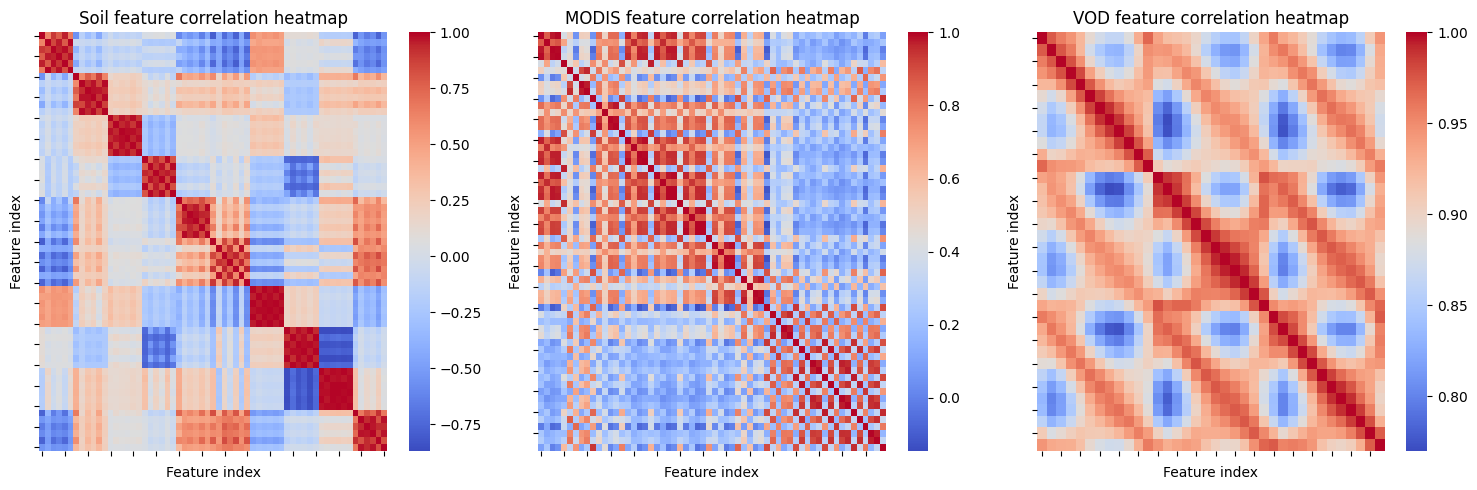
\includegraphics[width=0.9\textwidth]{assets/corr_hm.png}
    \caption{Correlation heatmap of the 3 biggest groups of geodata}
\end{figure}

Since these datasets individually can be broken down into groups of features generally talking about a similar topic we can see that the correlation within these groups is quite high. Even though previous work \cite{DBLP:journals/corr/abs-2007-00062} has demonstrated the viability of neural network models to learn from high dimensional data, removing redundant features has in numerous instances been shown to improve model performance \cite{chen2022survey}. With this in mind we decided to apply a Principal Component Analysis (PCA) to the geodata to reduce the dimensionality of the data. We specified that the number of principle components should be such that 95\% of the variance is explained.   

\subsection{Data preparation}

% talk about the augmentation 
Our training and test image instance - consisting of science citizen photographs - where taken by a wide variety of people under a wide variety of conditions. This means that the images are of varying quality, resolution, and orientation. We can see this just taking a random sample of 5 images.
\begin{figure}[!h]
    \centering
    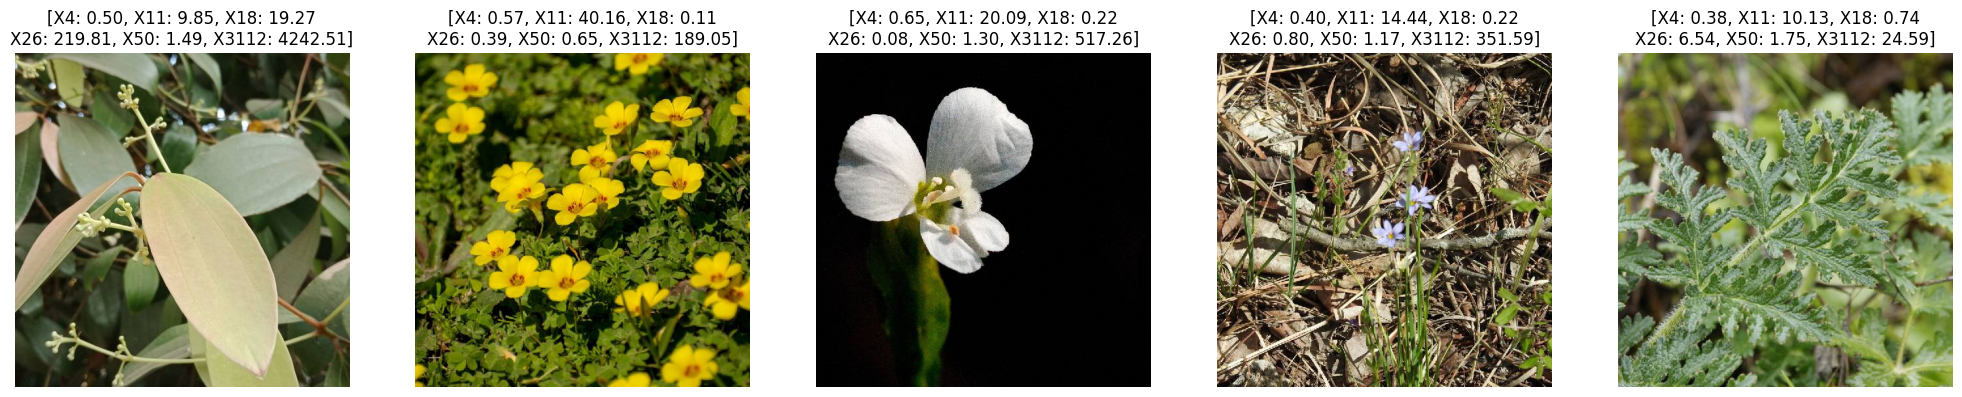
\includegraphics[width=0.9\textwidth]{assets/before_aug_img.png}
    \caption{Random sample of 5 images before augmentation annotated with their target trait labels}
\end{figure}

To prevent our model from fitting to noise in the data as a byproduct of how images where taken we decided to apply different keras preprocessing layers to batches concurrently. A key benefit of this would be that the model can generalize better to unseen data by learning potentially more meaningful features. While this approach of applying augmentations in the preprocessing stage is less flexible than having filters integrated in the model it does reduce model complexity though at the cost of potentially losing some ability to learn more complex features. Sampling again we can look at the results of our augmentaions. 

\begin{figure}[!h]
    \centering
    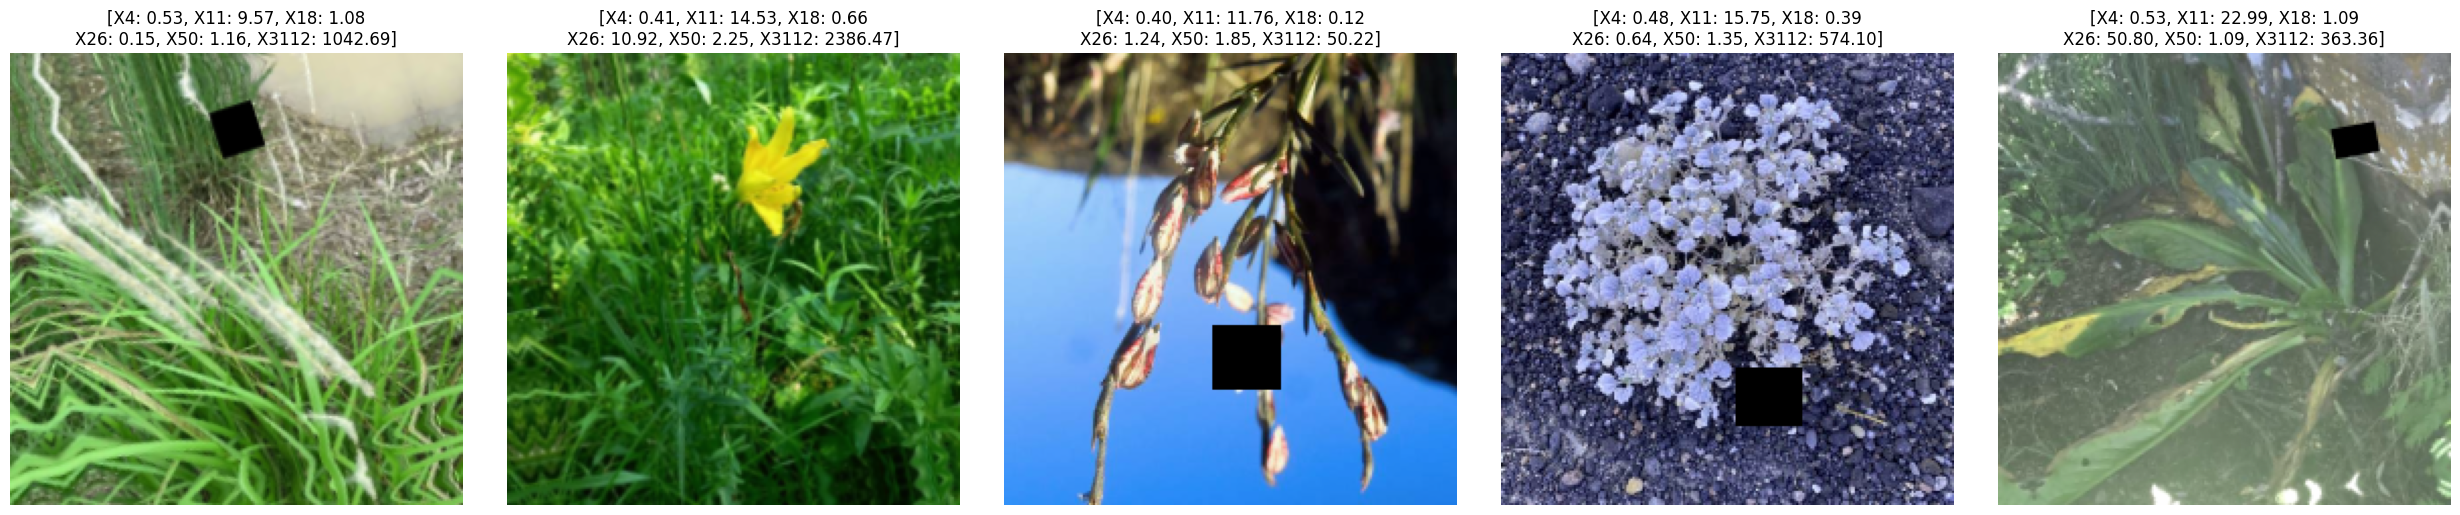
\includegraphics[width=0.9\textwidth]{assets/after_aug_img.png}
    \caption{Random sample of 5 images with augmentations: brightness, rotation, contrast, zoom, hue, cutout, flip, blur, saturation}
\end{figure}

% 5-fold stratified cross-validation + verification and split 
% \cite{Marcot2021} k = 5 good for large sample
% \cite{kequal10isgood} k ~ 10 generally good choice
Another method of reducing overfitting we thought relevant to apply here would be k-fold cross validation. For the choice of $k$ we chose 5 as for large datasets this has proven effective \cite{Marcot2021} and is generally around the commonly chosen value of 10 \cite{kequal10isgood}. Given that the data is from a geographically large enough sample we decided to create the folds in a stratified manner under the assumption the distribution of traits would be reasonably representaitive of the true distribution and thus one the model should learn. This is important as it ensures that the model is trained on a representative sample of the data in each fold and in turn has its predictions distributed in a similar manner to the assumed true distribution of the traits. So we reduce the risk of overfitting to the training data while also ensuring the model is trained using a representaitive sample of targets in each fold. To validate that the distributions of the target traits are indeed similar we averaged the distributions of the target traits in each fold and overlayed this on the original distribution of trait means and normalized them to the same scale. 

\begin{figure}[!h]
    \centering
    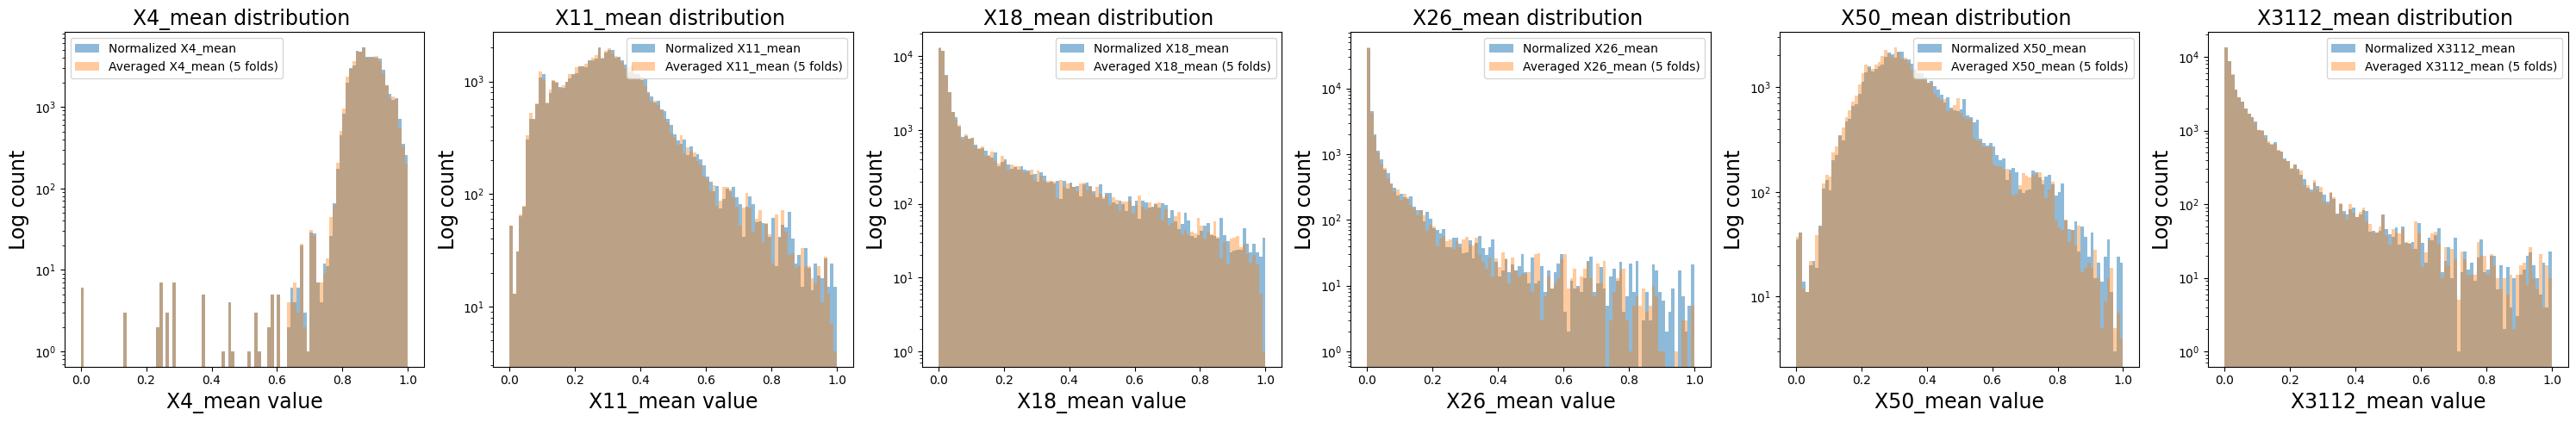
\includegraphics[width=1\textwidth]{assets/distribution_match_folds.png}
    \caption{Comparison of the average trait distributions in each fold with the original distribution of trait means ; (blue) normalized distribution of the trait means across the entire dataset ; (yellow) average normalized distribution of the trait means in each fold}
\end{figure}

\subsection{Model design}

\subsubsection{CNN trained on images}

% give an overview of the model 
    % activation function 
    % batch size
    % optimizer 
    % epochs
Our image CNN is a multi-output model which takes in a tensor consisting of red, green, and blue channels with an image size of 224x224 pixels. The model consists of a pretrained backbone; in our instance we compared \textit{efficientnetv2\_b2\_imagenet}, \textit{efficientnetv2\_s\_imagenet}, and \textit{resnet50\_imagenet}. The backbone outputs then feed into a global average pooling layer, followed by 2 dense layers and a dropout layer connected to the two dense output layers for the main and auxillary task. The hidden layers use a ReLU activation function, the outputs use no activation function as the targets are continuous. The model is trained using the Adam optimizer with a learning rate of 1e-4, a batch size of 48 and for 12 epochs. Additionally we used the $R^2$ metric for both loss and evaluation of the model performance as this is a regression problem. Finally we used step-based for the learning rate schedule which is defined as follows
\[
    \text{lr} = \text{lr}_\text{max} \times d^{\floor*{\frac{e_d}{r}}}
\]
Where $e_d$ is the current epoch, $r$ is the step size (=2), and $d$ is the decay rate.

% talk about the backbones 
    % ResNet 
    % EfficientNet b2 
    % EfficientNet s
\smallskip
Residual Network (ResNet) \cite{he2016identity} introduced in 2016 is a deep learning model that is able to learn features from images. Most famously its known for mitigating the vanishing gradient problem through the introduction of identiy skip connections. We are using \text{ResNet50} which was trained on imagenet and consists of 48 convolution layers, in addition to a MaxPool and AveragePool layer. EfficientNetV2 \cite{tan2021efficientnetv2} is a family of CNNs from 2021 that have faster speeds than many previous models primarily by increasing image size during training and incorporating adaptive regularization to compensate for any potential accuracy loss. We are using \textit{efficientnetv2\_b2\_imagenet} and \textit{efficientnetv2\_s\_imagenet} which are pretrained on imagenet, with the ladder being a smaller (fewer parameters) version of the former. Comparing these backbones in a table we can get some overview of how they stack up as seen in \ref{tab:backbone_comparison}

To compare these backbones we trained 3 different models with the same architecture but different backbones. We also specified a contribution of 0.3 to the final loss of the auxillary task (as opposed to 1.0 for the main task) as to limit its impacts on the direction of training. A visual overview of the different models can be seen in \ref{fig:models_overview}. 

\begin{table}[!h]
    % ref for this table 
    
    \centering
    \begin{tabular}{@{}llll@{}}
    \toprule
    & EfficientNetV2 b2 & EfficientNetV2 s & ResNet50 \\ \midrule
    parameters              & 8.77M             & 20.33M           & 23.56M   \\
    imagenet top 5 accuracy & 94.9\%            & 96.7\%           & (missing)       \\ \bottomrule
\end{tabular}
\caption{Comparison of the different backbones and published top 5 accuracy on imagenet for the specific models}
\label{tab:backbone_comparison}
\end{table}

\begin{figure}[!h]
    \centering
    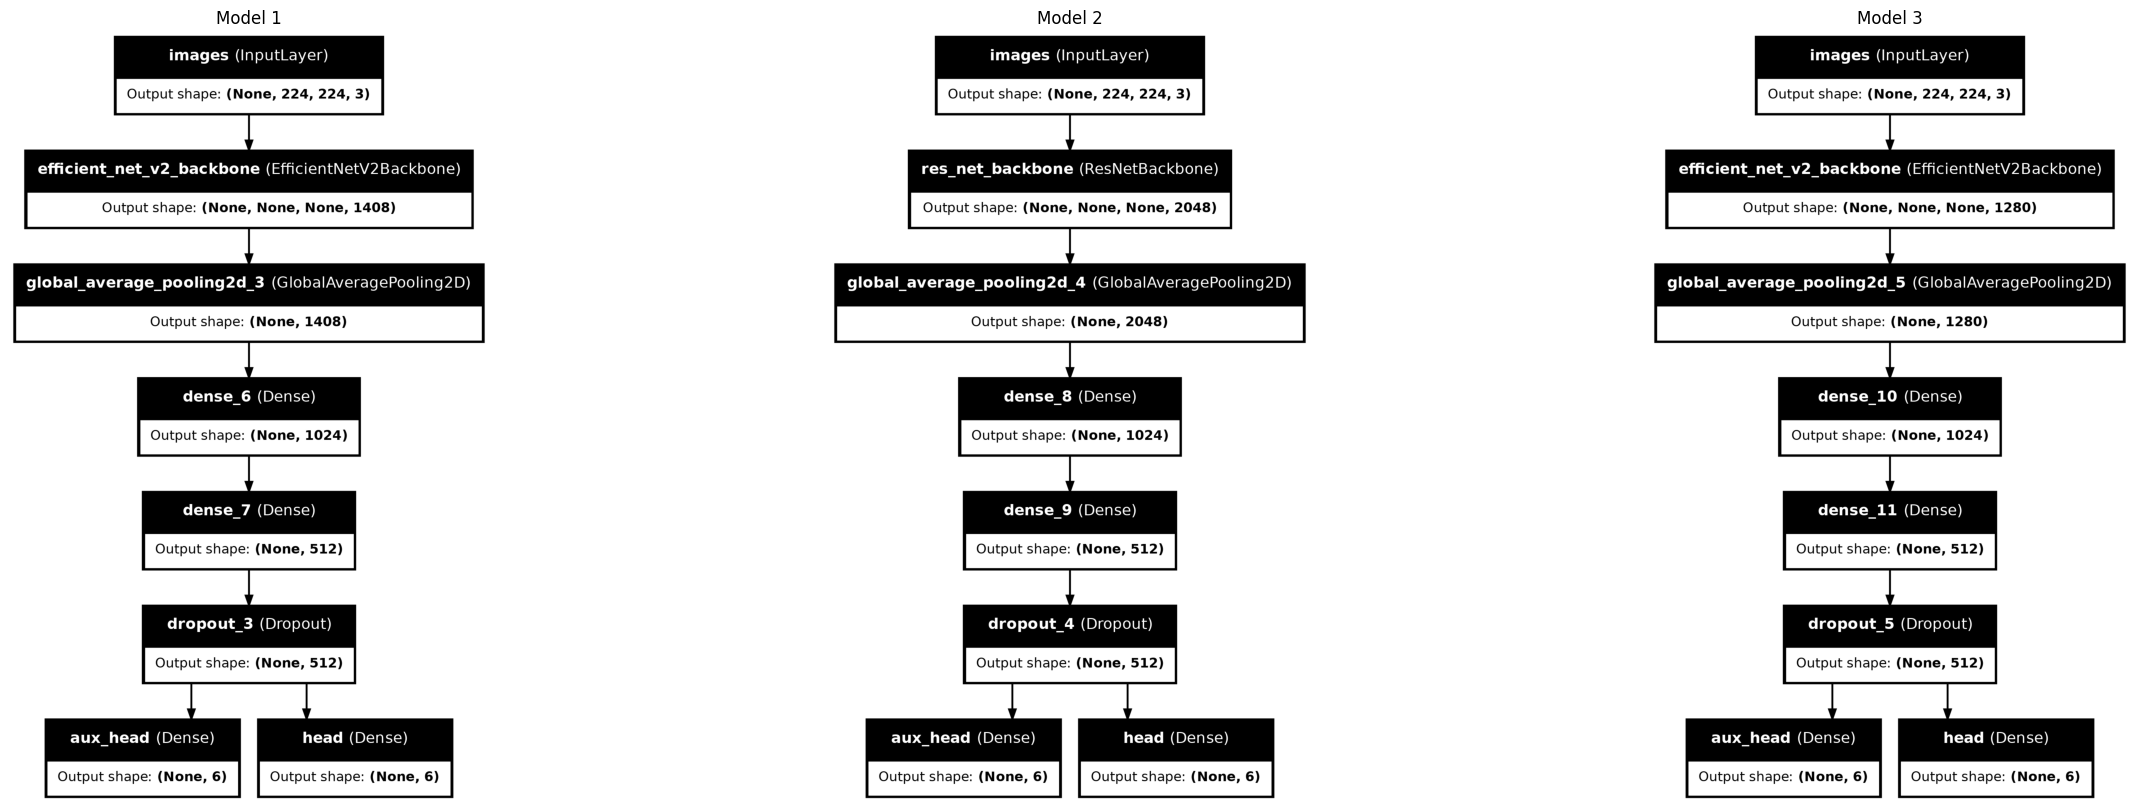
\includegraphics[width=1\textwidth]{assets/different_models.png}
    \caption{Visual overview of the 3 models with different backbones}
    \label{fig:models_overview}
\end{figure}

\subsubsection{CNN trained on images and geodata}

\subsection{Model evaluation}

% evaluation of individual models 

% comparative evaluation

\section{Results}

\section{Discussion}

\section{Conclusion}

\printbibliography

\end{document}